\section{CED}
\label{sec:chapter_4_section_3}
Il progetto di modellazione del CED (Centro Elaborazione Dati) sviluppato presso SOGEI, \`e stato realizzato con l'intento
di avere un modello 3D navigabile per consentire di sviluppare un sistema di Indoor Mapping e Indoor Navigation.
Sono stati sviluppati dei plugins coerenti con il contesto.
\newpage
Il primo gruppo di plugins sono importanti nel contesto della sicurezza degli edifici, infatti
(come si evince dalla Figura~\ref{fig:figura6}) essi sono: un estintore, un rilevatore di fumo, un naspo ed una
porta antincendio.
\begin{figure}[htbp]
\begin{center}
\begin{tabular}{c @{\hspace{1em}} c}
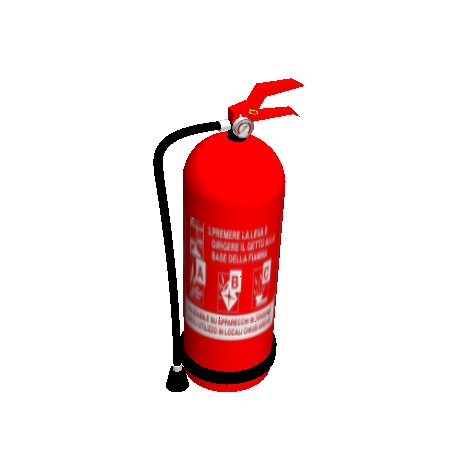
\includegraphics[width=5.5cm]{images/estintore} &
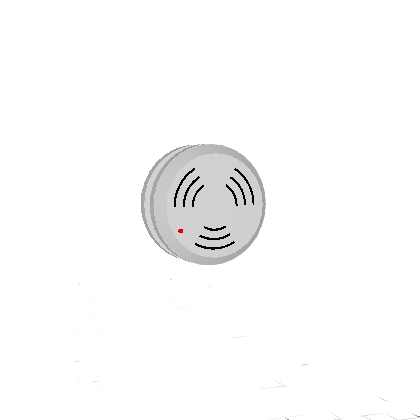
\includegraphics[width=5.5cm]{images/rilevatore} \\
 (a) & (b) \\
\end{tabular}
\begin{tabular}{c @{\hspace{1em}} c}
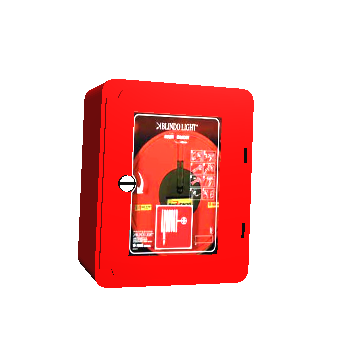
\includegraphics[width=5.5cm]{images/naspo} &
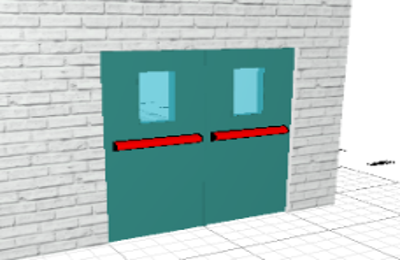
\includegraphics[width=5.5cm]{images/panicDoorDouble} \\
 (c) & (d) \\
\end{tabular}
\end{center}
\caption{Dettaglio Plugins: (a) estintore, (b) rilevatore fumo, (c) naspo, (d) porta antipanico}\label{fig:figura6}
\end{figure}
\newpage

Il secondo gruppo di plugins riguardano il contesto tecnologico (come si vede in Figura~\ref{fig:figura7}), essi sono
un metal detector, un rack server, un router wifi ed una telecamera.
\begin{figure}[htbp]
\begin{center}
\begin{tabular}{c @{\hspace{1em}} c}
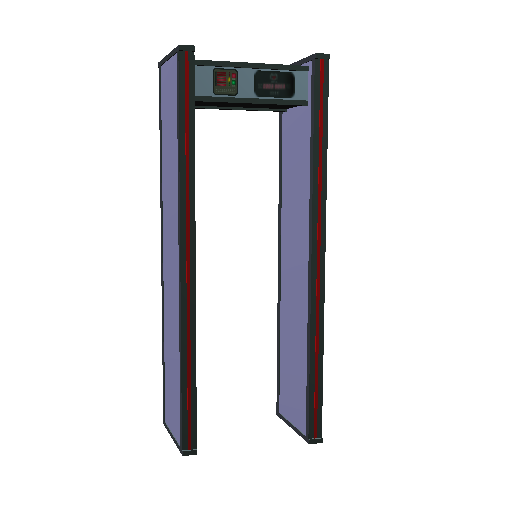
\includegraphics[width=5.5cm]{images/metalDetector} &
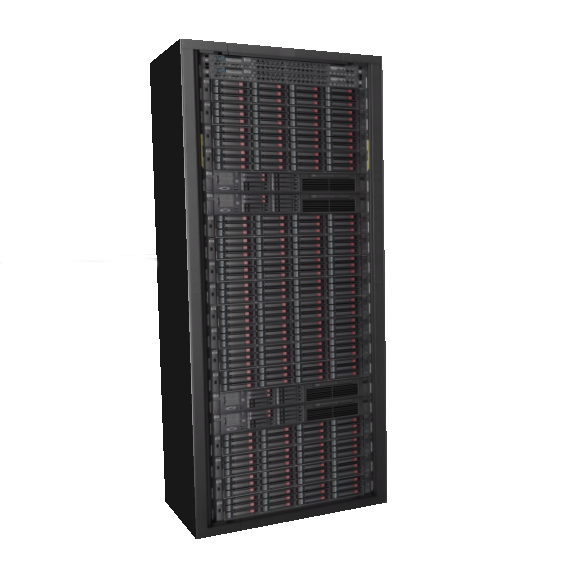
\includegraphics[width=5.5cm]{images/rack} \\
 (a) & (b) \\
\end{tabular}
\begin{tabular}{c @{\hspace{1em}} c}
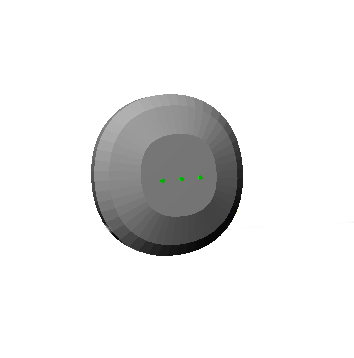
\includegraphics[width=5.5cm]{images/routerWifi} &
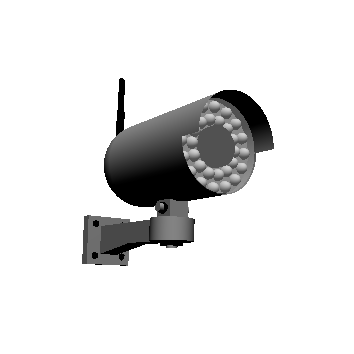
\includegraphics[width=5.5cm]{images/telecamera} \\
 (c) & (d) \\
\end{tabular}
\end{center}
\caption{Dettaglio Plugins: (a) metal detector, (b) rack server, (c) router wifi, (d) telecamera}\label{fig:figura7}
\end{figure}
